\documentclass[14pt]{beamer} 
\usetheme{default}

\usepackage{import}
\usepackage{graphicx}
\usepackage{amsmath}
\usepackage{amssymb}
\usepackage{amsthm}

\usepackage{tikz}
\usetikzlibrary{arrows}
\usetikzlibrary{shapes, arrows.meta}

\usepackage[absolute, overlay]{textpos}

\usepackage{pgfplots}
\usepackage[T1]{fontenc}
\usepackage{lmodern}
\usepackage[utf8]{inputenc}

\usepackage{caption}
\usepackage{subcaption}
\usepackage{../tex/mathpartir}

%\setbeamercovered{transparent}
\definecolor{bgcol}{rgb}{0.8, 0.8, 0.8}
\setbeamercolor{bgcolor}{fg=black,bg=bgcol}

\definecolor{green}{rgb}{0.0, 0.5, 0.0}
\definecolor{red}{rgb}{0.8, 0.0, 0.0}

\newcommand{\Type}{\mathsf{Type}}
\newcommand{\Space}{\mathsf{Space}}
\newcommand{\Open}{\mathsf{Open}}
\newcommand{\PLower}{\mathcal{P}_\lozenge}
\newcommand{\PUpper}{\mathcal{P}_\square}
\newcommand{\Prob}{\mathcal{R}}
\newcommand{\State}{\mathsf{State}}

\newcommand{\cov}{\vartriangleleft}
\newcommand{\nat}{\mathbb{N}}
\newcommand{\suchthat}{\ |\ }
\newcommand{\List}[1]{\mathsf{list}\ {#1}}
\newcommand{\rat}{\mathbb{Q}}
\newcommand{\R}{\mathbb{R}}
\newcommand{\bool}{\mathbb{B}}
\newcommand{\Prop}{\mathbb{P}}
\newcommand{\Dist}[1]{\mathcal{P}({#1})}
\newcommand{\fun}[2]{\lambda\ {#1}\Rightarrow{#2}}
\newcommand{\ret}[1]{\mathsf{ret}_{#1}}

\newcommand*\circled[1]{\tikz[baseline=(char.base)]{
            \node[shape=circle,draw,inner sep=2pt,thick] (char) {#1};}}
            
\newcommand{\dirsup}{\mathop{\setlength{\unitlength}{.7em}\raisebox{-.2em}%
    {\begin{picture}(1,1.5)\put(.5,0){\line(-1,3){.48}}
    \put(.5,0){\vector(1,3){.5}}\end{picture}}}} 
            
\newcommand*{\tikzbullet}[2]{%
  \setbox0=\hbox{\strut}%
  \begin{tikzpicture}
    \useasboundingbox (-.25em,0) rectangle (.25em,\ht0);
    \filldraw[draw=#1,fill=#2] (0,0.3\ht0) circle[radius=.25em];
  \end{tikzpicture}%
}

\newcommand{\SafeToGo}{\tikzbullet{green}{green}}
\newcommand{\SafeToStop}{\tikzbullet{red}{red}}

\title{Programming with continuous spaces}
%\author{\textbf{Ben Sherman}, Luke Sciarappa, Michael Carbin, Adam Chlipala}
\date{October 25, 2016}

\setbeamertemplate{footline}{%
  \raisebox{5pt}{\makebox[\paperwidth]{\hfill\makebox[10pt]{\scriptsize\insertframenumber}}}}
\setbeamertemplate{navigation symbols}{}

\begin{document}

\maketitle

\begin{frame}{Doing probability in Coq}
Probability distributions are over \emph{spaces}, not sets.

\bigskip
\pause

\begin{center}
\Huge Why?
\end{center}

\end{frame}

\begin{frame}{Assigning measure to arbitrary subsets?}

\begin{itemize}
\item Want to ``measure'' subsets (e.g., length, volume, probability)
\pause
\item Axiomatize how measure relates to subsets
\begin{itemize}
\item e.g., if $A \subseteq B$ then $\mu(A) \le \mu(B)$
\end{itemize}
\pause
\item Vitali (1905): (in ZFC) no way to consistently assign measure to all subsets of $\R$
\pause
\item Banach-Tarski paradox (1924): create two spheres from one with a discontinuous decomposition, then isometries
\end{itemize}
\end{frame}

\begin{frame}{Spaces, not sets}
\begin{itemize}
\item Sets aren't the right objects for measuring: \emph{spaces} are
\item Functions don't preserve spatial/measurement structure: \emph{continuous maps} do
\item If we want to write computer programs about probability, we need a PL for \emph{spaces} and \emph{continuous maps}
\end{itemize}
\end{frame}

\begin{frame}{But what are \emph{types}?}
\small

\begin{table}[]
\centering
\begin{tabular}{l | l l l}
model                & types are         & terms are                 & axioms              \\
\hline
classical            & sets              & functions                & LEM                 \\
realizability                  & tasks             & computer programs        & Church's law              \\
HoTT                 & $\infty$-grupoids & ``continuous maps''      & HITs, UA               \\
\textbf{topological} & \textbf{spaces}   & \textbf{continuous maps} & \textbf{continuity}
\end{tabular}
\end{table}

\end{frame}

\begin{frame}{PL for continuous spaces}

\begin{center}
{
\Large
\begin{align*}
\text{types} &\triangleq \text{spaces}
\\
\text{values} &\triangleq \text{points}
\\
\text{functions} &\triangleq \text{continuous maps}
\end{align*}
}
(But keep it computable, of course)
\end{center}
\end{frame}

\begin{frame}{Just add axioms to Coq?}
\begin{itemize}
\item Add continuity axioms to Coq, which refute LEM, so that types are spaces, not sets.
\item Problem: these axioms don't compute (and it'd be cool if they did).
\item Need to change computational interfaces of functions to fix it. 
\item Analogy: univalence doesn't compute in Coq, so build cubicaltt.
\end{itemize}
\end{frame}

\begin{frame}{$f$ must eventually ``ignore'' $x$}
\Large
\[
\frac{
f : (\nat \to \bool) \to \bool
\qquad
x : \nat \to \bool
}
{ f(x) : \bool }
\]
\end{frame}

\begin{frame}{Would like to compute...}
\[ f : (\nat \to \bool) \to \bool \]

Is $f([\mathsf{true}, \mathsf{false}])$ always $\mathsf{true}$? Is it ever $\mathsf{true}$?

\[ [ \mathsf{true}, \mathsf{false}] = \{ x : \nat \to \bool \suchthat x(0) = \mathsf{true}, x(1) = \mathsf{false} \} \]
\end{frame}

\begin{frame}
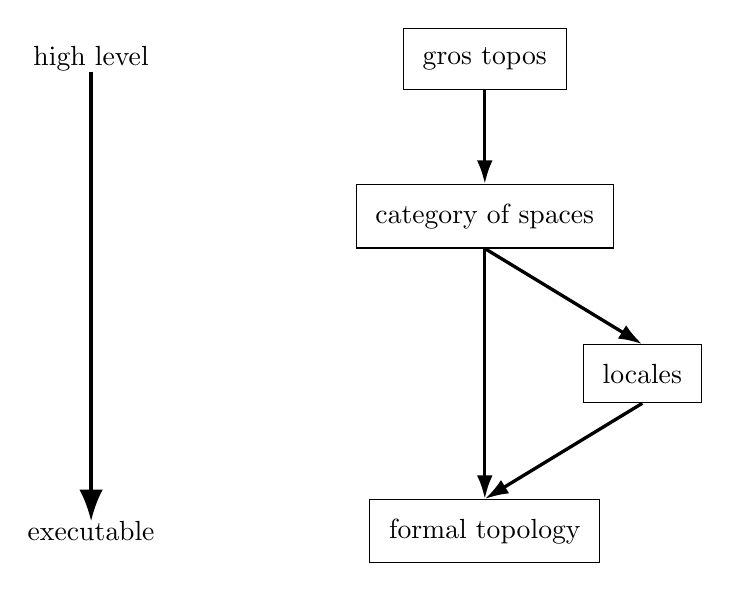
\begin{tikzpicture}
\node[inner sep=0pt] (highlevel) at (0,0)
  {high level};
\node[inner sep=0pt] (executable) at (0, -6)
  {executable};
\draw[-{Latex[length=4mm, width=3mm]},very thick] (highlevel.south) -- (executable.north);

\node[draw=black, rectangle, inner sep=7pt] (topos) at (5,0)
  {gros topos};
\node[draw=black, rectangle, inner sep=7pt] (cat) at (5,-2)
  {category of spaces};
\node[draw=black, rectangle, inner sep=7pt] (loc) at (7,-4)
  {locales};
\node[draw=black, rectangle, inner sep=7pt] (ft) at (5,-6)
  {formal topology};
  
\draw[-{Latex[length=3mm, width=2mm]},very thick] (topos.south) -- (cat.north);
\draw[-{Latex[length=3mm, width=2mm]},very thick] (cat.south) -- (loc.north);
\draw[-{Latex[length=3mm, width=2mm]},very thick] (cat.south) -- (ft.north);
\draw[-{Latex[length=3mm, width=2mm]},very thick] (loc.south) -- (ft.north);

\end{tikzpicture}
\end{frame}

\begin{frame}{Category of spaces}
Program with categorical operations, where objects are spaces and arrows are continuous maps.

\bigskip

Note: Given $A, B : \Space$, don't necessarily have the function space $A \Rightarrow B$!

\begin{align*}
\small
\frac
{\Gamma, A, B : \Space 
\qquad m : \Gamma \leadsto \Prob(A) 
\qquad f : \Gamma \times A \leadsto \Prob(B)}
{\mathsf{Bind}(m, f) : \Gamma \leadsto \Prob(B)}
\end{align*}
\end{frame}

\begin{frame}{Gros topos}

\begin{itemize}
\item Locally cartesian closed (has $\prod, \sum, \Rightarrow$)
\item Much like Coq (but no universes) 
\end{itemize}

\begin{align*}
\frac
{A, B : \Space}
{\mathsf{Bind} :: \widehat{\Prob(A)} \Rightarrow (\widehat{A} \Rightarrow \widehat{\Prob(B)}) \Rightarrow \widehat{\Prob(B)}}
\end{align*}

\end{frame}

\begin{frame}{Logic in sets vs. spaces}

\begin{table}[]
\small
\centering
\begin{tabular}{l | l | l}
model                & sets         & spaces    \\
\hline
$A : \_\_ $ & $\mathsf{Set}$ & $\Space$ \\
$U : A \to \Prop$ & subset & \emph{open} subspace \\
$\top$ & everything & everything \\
$\bot$ & nothing & nothing \\
infinitary $\vee$ & union & union \\
finite $\wedge$ & intersection & intersection \\
\hline \hline
$U \Rightarrow V$ & $\neg U \vee V$ & biggest $W$ such that $W \wedge U \subseteq V$ \\
$\neg$ & complement & biggest disjoint open subspace \\
$\bigwedge_{i : I} U_i$ & $\bigcap_{i : I} U_i$ & biggest $W$ such that ...
\end{tabular}
\end{table}
\end{frame}

\begin{frame}{Logic in spaces}
In $\R$,
\[
\neg (\cdot > 0) = \cdot < 0.
\]

Therefore,
\[
\top \nvdash \cdot < 0 \vee \neg (\cdot < 0).
\]
\end{frame}

\begin{frame}{Formal topology/locales}
\begin{itemize}
\item Explicit theory of topology which enables computation
\item Primitive definitions of spaces and continuous maps
\item Derivation of approximation rules
\end{itemize}
\end{frame}

\begin{frame}{Example approximation rules}
\[
\Downarrow : \Space \to \Type \to \Type
\]

\begin{mathpar}
\inferrule* [right=]
  {\varepsilon : \rat^+}
  {\R \Downarrow \rat}

\inferrule* [right=]
  {A \Downarrow I
  \\ B \Downarrow J}
  {A \times B \Downarrow I \times J}
  
\inferrule* [right=]
  { }
  {\mathsf{discrete}(I) \Downarrow I}
  
\inferrule* [right=]
  {A \Downarrow I}
  {\PLower^+(A) \Downarrow I}
\end{mathpar}
\end{frame}


\begin{frame}{Challenges}
\begin{itemize}
\item How to make low-level constructions possible at the highest level of abstraction?
\item Pain having to manually work with syntax
\begin{itemize}
\item e.g., $\mathsf{fst} \circ \langle f , g \rangle \Longrightarrow f$
\item Very painful at gros topos level (manual $\beta$-reduction)
\end{itemize}
\end{itemize}
\end{frame}

\end{document}

